\section{Presentación de un grupo}

En teoría de grupos, una \textbf{presentación de grupo} es una forma de describir un grupo mediante un conjunto de \textbf{generadores}, que producen todos los elementos del grupo, y un conjunto de \textbf{relaciones}, que imponen restricciones sobre cómo estos generadores interactúan. Se expresa simbólicamente como:
\[
\langle \text{generadores} \mid \text{relaciones} \rangle
\]
Esta notación proporciona una descripción compacta y útil para estudiar la estructura de los grupos, sin necesidad de enumerar todos sus elementos.ensin necesidad de describir explícitamente todos sus elementos.\\



Dado un conjunto \( X \), se denota por \( G_X \) al grupo libre generado por \( X \) y con $e$ denotaremos su elemento identidad. 




\begin{definicion}
	\upshape{
		Sean \( X \) un conjunto y \( R \subseteq G_X \) un subconjunto. Decimos que un grupo \( G \) está definido por los generadores en \( X \) y las relaciones \( w = e \),\( w \in R \), si
		\[
		G \cong G_X / N_R,
		\]
		donde \( N_R \) es el subgrupo normal de \( G_X \) generado por \( R \).
		
		\medskip
		
		\noindent En este caso, denotamos
		\[
		 G_X / N_R:= \langle X : w = e,\ w \in R \rangle \quad \text{o bien} \quad \langle X : R \rangle.
		\]
		Y se le denomina \emph{presentación} de \( G \).
	}
\end{definicion}


\begin{observacion}
	\upshape{
		Las relaciones \( w = e \), \( w \in R \), consisten en que para todo \( w \in R \) se tiene que \( w N_R = N_R = e N_R \); es decir, indican que los elementos \( w \in R \), considerados como clases, corresponden a la identidad en \( \langle X : R \rangle \).
	}
\end{observacion}

\begin{observacion}
	\upshape{
		Si \( X = \varnothing \), entonces el grupo libre generado por \( X \) es el grupo trivial:
		\[
		G_X = \{e\}.
		\]
		En consecuencia, para cualquier conjunto de relaciones \( R \subseteq G_X \), se tiene que \( N_R = \{e\} \), y por tanto
		\[
		G_X / N_R = \{eN_R\} = \{N_R\},
		\]
		lo cual significa que se trata de un grupo trivial.
		
		\medskip
		
		\noindent Por tanto, \( \langle \emptyset : R \rangle \) es la presentación de todo grupo trivial.
	}
\end{observacion}

Habiendo establecido la definición y notación de presentación de un grupo, la pregunta natural es cómo construirlas. El método principal para obtener presentaciones consiste en usar la propiedad universal del grupo libre junto con el teorema fundamental del homomorfismo de grupos. A continuación, el Ejemplo \ref{poiuyt} ilustrará este proceso con detalle.

\begin{ejemplo}\label{poiuyt}
	\upshape{
	
		El grupo ciclico $$\dfrac{\mathbb{Z}}{n\mathbb{Z}}=\{\:\overline{0},\overline{1},\overline{2},\cdots, \overline{n-1}\:\}$$ se puede escribir como $\langle x: x^n=e\rangle$.
	}
\end{ejemplo}


\begin{proof}[Justificación]
	Consideremos \( X := \{x\} \) y la función 
	\begin{align*}
		j : X &\longrightarrow \dfrac{\mathbb{Z}}{n\mathbb{Z}}\\[4pt]
		x &\longmapsto \overline{1}.
	\end{align*}
	Por la propiedad universal del grupo libre, existe un único homomorfismo de grupos \( f : G_X \to \mathbb{Z}/n\mathbb{Z} \) tal que \( f \circ \iota = j \):
	\[
	\xymatrix{
		X \ar[rr]^{\displaystyle j} \ar@{^(->}[dd]_{\displaystyle \iota } & & \dfrac{\mathbb{Z}}{n\mathbb{Z}} \\
		&&\\
		G_X \ar@{-->}[rruu]_{\displaystyle \exists !f} &&
	}
	\]  
	De donde se tiene que 
	\begin{align*}
		f : G_X &\longrightarrow \dfrac{\mathbb{Z}}{n\mathbb{Z}} \\[4pt]
		[x]^m &\longmapsto m\;\overline{1}.
	\end{align*}
	Ya que como \( f \) es un homomorfismo de grupos, se cumple que 
	\[
	f\left([x]^m\right) = mf\left([x]\right)= m\left((f\circ \iota)(x)\right) = mj(x) = m\;\overline{1}.
	\] Además es fácil ver que es sobreyectivo. Luego, por el teorema fundamental del homomorfismo de grupos, se tiene que 
	\[
	\dfrac{G_{X}}{\ker f} \cong \dfrac{\mathbb{Z}}{n\mathbb{Z}},
	\]
	por lo que nos interesa ahora saber cómo es el núcleo de \( f \). 
	\begin{align*}
		\ker f &= \left\{\:[x]^m : f([x]^m) = \overline{0}\:\right\}\\[4pt]
		&= \{\:[x]^m : m\;\overline{1} = \overline{0}\:\}\\[4pt]
		&= \{\:[x]^m : m \text{ es múltiplo de } n\:\}\\[4pt]
		&= \langle [x]^n \rangle.
	\end{align*} 
	Así, tenemos \( X = \{x\} \) y consideramos \( R = \{[x]^n\} \subset G_X \); podemos verificar facilmente que, \( N_R = \langle [x]^n\rangle\), y por definición se tiene que  
	\[
	\dfrac{G_{X}}{\ker f} = \dfrac{G_{\{x\}}}{\langle [x]^n \rangle} =: \langle x : [x]^n = e \rangle.
	\] 	Por otro lado, notemos que \( [x] = x \), pues \( x \) es una palabra reducida (no se puede reducir más). Entonces se tiene, por igualdad de conjuntos, que 
	\[
	\langle x : [x]^n = e \rangle = \langle\, x : x^n = e\, \rangle.
	\] 	Por lo tanto, finalmente obtenemos
	\[
	\dfrac{\mathbb{Z}}{n\mathbb{Z}} \cong \langle \,x : x^n = e \,\rangle
	\]
\end{proof}




\begin{ejemplo}
	\upshape{
		El grupo de los números enteros $\mathbb{Z}$ se puede escribir como $\langle x : \emptyset \rangle$.
	}
\end{ejemplo}

\begin{proof}[Justificación]
	Consideremos \( X := \{x\} \) y la función 
	\begin{align*}
		j : X &\longrightarrow \mathbb{Z}\\[4pt]
		x &\longmapsto 1.
	\end{align*}
	Por la propiedad universal del grupo libre, existe un único homomorfismo de grupos \( f : G_X \to \mathbb{Z} \) tal que \( f \circ \iota = j \):
	\[
	\xymatrix{
		X \ar[rr]^{\displaystyle j} \ar@{^(->}[dd]_{\displaystyle \iota } & & \mathbb{Z} \\
		&&\\
		G_X \ar@{-->}[rruu]_{\displaystyle \exists !f} &&
	}
	\]	
	De donde se tiene que 
	\begin{align*}
		f : G_X &\longrightarrow \mathbb{Z} \\[4pt]
		[x]^m &\longmapsto m \cdot 1 = m.
	\end{align*}	
	Ya que como \( f \) es un homomorfismo de grupos, se cumple que 
	\[
	f\left([x]^m\right) = m f\left([x]\right) = m\left((f\circ \iota)(x)\right) = m j(x) =  m1 = m.
	\]Además es sobreyectivo. Luego, por el teorema fundamental del homomorfismo de grupos, se tiene que 
	\[
	\dfrac{G_{X}}{\ker f} \cong \mathbb{Z},
	\]
	por lo que nos interesa ahora saber cómo es el núcleo de \( f \). 
	\begin{align*}
		\ker f &= \left\{\:[x]^m : f([x]^m) = 0\:\right\}\\[4pt]
		&= \{\:[x]^m : m = 0\:\}\\[4pt]
		&= \{\:[x]^0 \:\}\\[4pt]
		&=\{[e]\}=\{e\}\\[4pt]
		&= \langle e \rangle.
	\end{align*}	
	Así, tenemos \( X = \{x\} \) y consideramos \( R = \emptyset \subset G_X \); esto es, \( N_R = \ker f \), y por definición se tiene que 	
	\[
	\dfrac{G_{X}}{\ker f} = \dfrac{G_{\{x\}}}{\langle e \rangle} =:\langle x : w=e,w\in R \rangle= \langle x : \emptyset \rangle.
	\] 	Por lo tanto, obtenemos
	\[
	\mathbb{Z} \cong \langle \,x : \emptyset \,\rangle.
	\]
\end{proof}


\section{Grupo simétrico}


Una permutación es, en esencia, una reordenación de los elementos de un conjunto. Podemos entenderla formalmente como una función biyectiva.

\begin{definicion}
	\upshape{
		Sea \( X \) un conjunto no vacío. Una función \(\sigma : X \to X\) biyectiva se
		denomina permutación del conjunto \( X \).
	}
\end{definicion}

La composición de biyecciones del conjunto \( X \) vuelve a ser una biyección, y la función identidad es una biyección. Además, toda biyección tiene inversa que también es biyección. Así, se cumple que:

\begin{itemize}
	\item La composición de permutaciones es una operación interna.
	\item La composición es asociativa.
	\item La función identidad es la permutación identidad.
	\item Dada \(\sigma\) una permutación, entonces la función inversa \(\sigma^{-1}\) es la permutación inversa.
\end{itemize}

Por lo que tenemos una estructura de grupo.

\begin{definicion}
	\upshape{
		El conjunto de todas las permutaciones (biyecciones) de un conjunto \( X \) con la composición de funciones forma un grupo llamado \textit{grupo de permutaciones} (grupo de biyecciones), denotado por
		\[
		\operatorname{Biyec}(X).
		\]
	}
\end{definicion}

\begin{definicion}
	\upshape{
		Si el conjunto \( X \) es un subconjunto de los números naturales, es decir,
		\[
		X = \{1, 2, \ldots, n\},
		\]
		entonces su correspondiente grupo de permutaciones \(\operatorname{Biyec}(X)\) se denomina \emph{grupo simétrico} de \(n\) elementos y se denota usualmente como \(S_n\) o también como \(\Sigma_n\).
		
		\medskip
		\noindent
		A los elementos del grupo simétrico se les denomina \emph{permutaciones de \(n\) letras}.
	}
\end{definicion}

\begin{observacion}
	\upshape
	El grupo simétrico \(\Sigma_n\) tiene  orden \(n!\).
\end{observacion}



\begin{ejemplo}
	\upshape
	Sea \(X = \{1; 2\}\). Entonces, las únicas permutaciones de \(X\) son:
	\[
	\begin{array}{rcl}
		\sigma_1: & X \to X & \\
		& 1 \mapsto 1, & \\
		& 2 \mapsto 2 &
	\end{array}
	\qquad \text{y} \qquad
	\begin{array}{rcl}
		\sigma_2: & X \to X & \\
		& 1 \mapsto 2, & \\
		& 2 \mapsto 1 &
	\end{array}
	\]
	Con lo cual, \(\Sigma_2 = \{\sigma_1, \sigma_2\}\). Más aún, un elemento \(\sigma \in \Sigma_2\) queda determinado por su imagen, y podemos escribir:
	\[
	\sigma = \left(\begin{array}{cc}
		1 & 2 \\
		\sigma(1) & \sigma(2)
	\end{array}\right).
	\]
	En este caso:
	\[
	\sigma_1 = \left(\begin{array}{cc}
		1 & 2 \\
		1 & 2
	\end{array}\right)
	\qquad \text{y} \qquad
	\sigma_2 = \left(\begin{array}{cc}
		1 & 2 \\
		2 & 1
	\end{array}\right). 
	\]
\end{ejemplo}

\medskip
\begin{observacion}
	\upshape{
		Note que $\sigma_1\sigma_2=\sigma_2\sigma_1$ por lo que $\Sigma_2$ es un grupo abeliano.
	}
\end{observacion}

\medskip
\begin{ejemplo}
	\upshape{
		Sea \(X = \{1, 2, 3\}\). Entonces, \(\Sigma_3\) tiene \(3! = 6\) elementos:
		
		
		\[
		I = \left(\begin{array}{ccc}
			1 & 2 & 3 \\
			1 & 2 & 3
		\end{array}\right), \quad
		\alpha = \left(\begin{array}{ccc}
			1 & 2 & 3 \\
			2 & 3 & 1
		\end{array}\right), \quad
		\alpha' = \left(\begin{array}{ccc}
			1 & 2 & 3 \\
			3 & 1 & 2
		\end{array}\right),
		\]
		\[
		\beta = \left(\begin{array}{ccc}
			1 & 2 & 3 \\
			3 & 2 & 1
		\end{array}\right), \quad
		\beta' = \left(\begin{array}{ccc}
			1 & 2 & 3 \\
			1 & 3 & 2
		\end{array}\right), \quad
		\beta'' = \left(\begin{array}{ccc}
			1 & 2 & 3 \\
			2 & 1 & 3
		\end{array}\right).
		\]
		
		\medskip
		\noindent Además, observamos que:
		\begin{align*}
			\alpha^2 &= \alpha \alpha = \left(\begin{array}{ccc}
				1 & 2 & 3 \\
				3 & 1 & 2
			\end{array}\right) = \alpha', \\[1ex]
			\alpha^3 &= \alpha \alpha^2 = \left(\begin{array}{ccc}
				1 & 2 & 3 \\
				1 & 2 & 3
			\end{array}\right) = I, \\[1ex]
			\alpha \beta &= \left(\begin{array}{ccc}
				1 & 2 & 3 \\
				1 & 3 & 2
			\end{array}\right) = \beta', \\[1ex]
			\alpha^2 \beta &= \left(\begin{array}{ccc}
				1 & 2 & 3 \\
				2 & 1 & 3
			\end{array}\right) = \beta''.
		\end{align*}
		Por lo tanto, 
		\[
		\Sigma_3 = \{I, \alpha, \alpha^2, \beta, \alpha \beta, \alpha^2 \beta\}.
		\]
	}
\end{ejemplo}

\begin{observacion}
	\upshape{
		Podemos obtener la siguiente tabla de operaciones de los elementos del grupo simétrico $\Sigma_3$.
		\begin{table}[H]
			\centering
			{\large
				\renewcommand{\arraystretch}{2.2}% Aumenta el espacio entre filas
				\resizebox{160mm}{!}{
					\begin{tabular}{
							>{\centering\arraybackslash}p{3cm}
							>{\centering\arraybackslash}p{3cm}
							>{\centering\arraybackslash}p{3cm}
							>{\centering\arraybackslash}p{3cm}
							>{\centering\arraybackslash}p{3cm}
							>{\centering\arraybackslash}p{3cm}
							>{\centering\arraybackslash}p{3cm}
						}
						\toprule
						$\scalebox{1.5}{$\circ$}$ & $\scalebox{1.5}{$I$}$ & $\scalebox{1.5}{$\alpha$}$ & $\scalebox{1.5}{$\alpha^2$}$ & $\scalebox{1.5}{$\beta$}$ & $\scalebox{1.5}{$\alpha\beta$}$ & $\scalebox{1.5}{$\alpha^2\beta$}$ \\
						\midrule
						$\scalebox{1.5}{$I$}$ & $\scalebox{1.5}{$I$}$ & $\scalebox{1.5}{$\alpha$}$ & $\scalebox{1.5}{$\alpha^2$}$ & $\scalebox{1.5}{$\beta$}$ & $\scalebox{1.5}{$\alpha\beta$}$ & $\scalebox{1.5}{$\alpha^2\beta$}$ \\
						$\scalebox{1.5}{$\alpha$}$ & $\scalebox{1.5}{$\alpha$}$ & $\scalebox{1.5}{$\alpha^2$}$ & $\scalebox{1.5}{$I$}$ & $\scalebox{1.5}{$\alpha\beta$}$ & $\scalebox{1.5}{$\alpha^2\beta$}$ & $\scalebox{1.5}{$\beta$}$ \\
						$\scalebox{1.5}{$\alpha^2$}$ & $\scalebox{1.5}{$\alpha^2$}$ & $\scalebox{1.5}{$I$}$ & $\scalebox{1.5}{$\alpha$}$ & $\scalebox{1.5}{$\alpha^2\beta$}$ & $\scalebox{1.5}{$\beta$}$ & $\scalebox{1.5}{$\alpha\beta$}$ \\
						$\scalebox{1.5}{$\beta$}$ & $\scalebox{1.5}{$\beta$}$ & $\scalebox{1.5}{$\alpha^2\beta$}$ & $\scalebox{1.5}{$\alpha\beta$}$ & $\scalebox{1.5}{$I$}$ & $\scalebox{1.5}{$\alpha^2$}$ & $\scalebox{1.5}{$\alpha$}$ \\
						$\scalebox{1.5}{$\alpha\beta$}$ & $\scalebox{1.5}{$\alpha\beta$}$ & $\scalebox{1.5}{$\beta$}$ & $\scalebox{1.5}{$\alpha^2\beta$}$ & $\scalebox{1.5}{$\alpha$}$ & $\scalebox{1.5}{$I$}$ & $\scalebox{1.5}{$\alpha^2$}$ \\
						$\scalebox{1.5}{$\alpha^2\beta$}$ & $\scalebox{1.5}{$\alpha^2\beta$}$ & $\scalebox{1.5}{$\alpha\beta$}$ & $\scalebox{1.5}{$\beta$}$ & $\scalebox{1.5}{$\alpha^2$}$ & $\scalebox{1.5}{$\alpha$}$ & $\scalebox{1.5}{$I$}$ \\
						\bottomrule
					\end{tabular}
			}}
			\caption{Tabla de operaciones del grupo simétrico \(\Sigma_3\).}
		\end{table}
		\noindent De esta tabla podemos ver que $\Sigma_3$ no es un grupo abeliano, pues existe al menos un par de elementos que no conmutan:
		
		\[
		\alpha \beta =
		\left(
		\begin{array}{ccc}
			1 & 2 & 3 \\ 
			3 & 1 & 2
		\end{array}
		\right)
		\neq 
		\left(
		\begin{array}{ccc}
			1 & 2 & 3 \\ 
			2 & 3 & 1
		\end{array}
		\right)
		= \beta \alpha.
		\]
		
	}
\end{observacion}

\medskip
\begin{proposicion}
	\upshape{
		El grupo simétrico \(\Sigma_n\) es abeliano si \(n = 2\) y  es no abeliano si \(n \geq 3\).
	}
\end{proposicion}

\begin{proof}
	Si \(n = 2\), entonces \(\Sigma_2\) contiene solo dos permutaciones:
	\[
	I = \left(\begin{array}{cc}
		1 & 2 \\
		1 & 2
	\end{array}\right),
	\qquad
	\sigma = \left(\begin{array}{cc}
		1 & 2 \\
		2 & 1
	\end{array}\right).
	\]
	Como \(I \sigma = \sigma I = \sigma\), se concluye que \(\Sigma_2\) es abeliano.
	
	\medskip
	\noindent Supongamos ahora que \(n \geq 3\). Definimos dos permutaciones en \(\Sigma_n\):
	\[
	\sigma = \left(\begin{array}{ccccccc}
		1 & 2 & 3 & 4 & \cdots & n \\
		2 & 3 & 1 & 4 & \cdots & n
	\end{array}\right),
	\qquad
	\rho = \left(\begin{array}{ccccccc}
		1 & 2 & 3 & 4 & \cdots & n \\
		1 & 3 & 2 & 4 & \cdots & n
	\end{array}\right).
	\]
	Estas permutaciones actúan no trivialmente solo sobre las posiciones \(1\), \(2\) y \(3\), dejando fijas las demás.
	Entonces:
	\[
	\sigma\rho = \left(\begin{array}{ccccccc}
		1 & 2 & 3 & 4 & \cdots & n \\
		2 & 1 & 3 & 4 & \cdots & n
	\end{array}\right)\quad\text{y}\quad
	\rho\sigma = \left(\begin{array}{ccccccc}
		1 & 2 & 3 & 4 & \cdots & n \\
		3 & 2 & 1 & 4 & \cdots & n
	\end{array}\right).
	\]
	
	\medskip
	\noindent Como
	\[
	\sigma\rho \neq \rho\sigma,
	\]
	se concluye que \(\Sigma_n\) no es abeliano para \(n \geq 3\).
\end{proof}

Escribir una permutación \(\sigma \in \Sigma_n\) como  
\[
\sigma = \left(\begin{array}{ccccccc}
	1 & 2 & 3 & 4 & \cdots & n \\
	\sigma(1) & \sigma(2) & \sigma(3) & \sigma(4) & \cdots & \sigma(n)
\end{array}\right)
\]
resulta redundante, ya que siempre se repite la primera fila de manera fija. Por esta razón, se introduce una notación más eficiente y concisa conocida como \textit{notación cíclica}.

\medskip
\noindent Para comprender esta nueva forma de denotar permutaciones, consideremos el siguiente ejemplo:
\[
\sigma = \left(\begin{array}{cccccccc}
	1 & 2 & 3 & 4 & 5 & 6 & 7 & 8 \\
	4 & 2 & 7 & 5 & 1 & 8 & 6 & 3
\end{array}\right)\in \Sigma_8.
\]

\noindent Las imágenes sucesivas de \(1\) mediante \(\sigma\) son:
\[
\sigma^0(1) = 1,\quad \sigma(1) = 4,\quad \sigma^2(1) = 5,\quad \sigma^3(1) = 1,\quad \text{y} \quad \sigma^j(1) = \sigma^{j-3}(1)\text{ para }j \geq 4.
\]
Entonces, estas imágenes sucesivas de \(1\) mediante \(\sigma\) se escriben en forma cíclica como:
\[
\sigma_1 := (\:1\quad 4\quad 5\:).
\]

\noindent Tomamos ahora el menor elemento de \(\{1,2,3,\dots,n\}\), con \(n = 8\), que no esté en el conjunto \(\{1,4,5\}\). Ese elemento es \(2\), y sus imágenes mediante \(\sigma\) son:
\[
\sigma^0(2) = 2,\quad \sigma(2) = 2,
\]
por lo tanto, escribimos:
\[
\sigma_2 := (2).
\]

\noindent De modo similar, tomamos el menor elemento que no está en \(\{1,2,4,5\}\), es decir, \(3\), y calculamos:
\[
\sigma^0(3) = 3,\quad \sigma(3) = 7,\quad \sigma^2(3) = 6,\quad \sigma^3(3) = 8,\quad \sigma^4(3) = 3,
\]
lo que se denota cíclicamente como:
\[
\sigma_3 := (\:3\quad 7\quad 6\quad 8\:).
\]

\noindent Finalmente, se intentaría continuar con el siguiente menor elemento que no está en \(\{1,2,3,4,5,6,7,8\}\), pero ya no quedan más elementos. Por lo tanto, hemos terminado el proceso y podemos escribir:
\[
\sigma = \sigma_3 \sigma_2 \sigma_1.
\]
\noindent A cada \(\sigma_j\) se le denomina \emph{ciclo}, y la función \(k \mapsto \sigma_j(k)\) se define así: si el ciclo es
\[
\sigma_j = (\:a_1\quad a_2\quad a_3\quad\cdots\quad a_r\:), \quad r \leq n,
\]
entonces, para \(k \in \{1,2,\dots,n\}\), se define:
\[
\sigma_j(k) := \begin{cases}
	a_{s+1} & \text{si } k = a_s \in \{a_1, a_2, \dots, a_{r-1}\}, \\
	a_1     & \text{si } k = a_r, \\
	k       & \text{si } k \notin \{a_1, a_2, \dots, a_r\}.
\end{cases}
\]

\noindent Así, por ejemplo:
\begin{itemize}
	\item \(\sigma(1) = \sigma_3\sigma_2\sigma_1(1) = 4\), porque en el ciclo \(\sigma_1 = (1\ 4\ 5)\), el número que sigue a \(1\) es \(4\); además, \(\sigma_2(4) = 4\) y \(\sigma_3(4) = 4\).
	\item \(\sigma(4) = \sigma_3\sigma_2\sigma_1(4) = 5\), porque en el ciclo \((1\ 4\ 5)\), el número que sigue a \(4\) es \(5\).
	\item \(\sigma(5) = \sigma_3\sigma_2\sigma_1(5) = 1\), porque en el ciclo \((1\ 4\ 5)\), el número que sigue a \(5\) es \(1\).
	\item \(\sigma(2) = \sigma_3\sigma_2\sigma_1(2) = 2\), porque el ciclo \(\sigma_2 = (2)\) deja a \(2\) fijo.
	\item \(\sigma(3) = 7\), \(\sigma(7) = 6\), \(\sigma(6) = 8\) y \(\sigma(8) = 3\), por lectura directa del ciclo \((3\ 7\ 6\ 8)\).
\end{itemize}

y recupereamos \[
\sigma =\sigma_3\sigma_2\sigma_1= \left(\begin{array}{cccccccc}
	1 & 2 & 3 & 4 & 5 & 6 & 7 & 8 \\
	4 & 2 & 7 & 5 & 1 & 8 & 6 & 3
\end{array}\right)\in \Sigma_8.
\]


\begin{observacion}
	\upshape{
		Cuando un ciclo es trivial, como en el caso de \(\sigma_2 = (2)\), se suele omitir en la notación cíclica. Por tanto, simplemente escribiremos:
		\[
		\sigma = \sigma_3 \sigma_2 \sigma_1 = \sigma_3 \sigma_1.
		\]
		O más simple aún, podemos escribir directamente:
		\[
		\sigma = (\:3\quad 7\quad 6\quad 8\:)(\:1\quad 4\quad 5\:).
		\]
	}
\end{observacion}

\begin{ejemplo}
	\upshape{
		La permutación \[
		\alpha = \left(\begin{array}{cccccccc}
			1 & 2 & 3 & 4 & 5 & 6 \\
			3 & 1 & 4 & 2 & 6 & 5 
		\end{array}\right)\in \Sigma_6
		\] se escribe en notación ciclica de la forma $\alpha=(\:5\quad 6\:)(\:1\quad 3\quad 4\quad 2\:)$
	}
\end{ejemplo}

\begin{observacion}
	\upshape{
		En general dos ciclos no conmutan. Por ejemplo, en $\Sigma_6$ consideremos los ciclos $\beta_1=(\:1\quad 3\quad 5\:)$ y $\beta_2=(\:3\quad 5\quad 6\:)$ y se tiene que $\beta_2\beta_1\neq \beta_1\beta_2$ ya que
		\[
		\beta_2\beta_1 = \left(\begin{array}{cccccccc}
			1 & 2 & 3 & 4 & 5 & 6  \\
			5 & 2 & 6 & 4 & 1 & 3 
		\end{array}\right)=(\:3\quad 6\:)(\:1\quad 5\:)
		\]
		
		\[
		\beta_1\beta_2 = \left(\begin{array}{cccccccc}
			1 & 2 & 3 & 4 & 5 & 6  \\
			3 & 2 & 1 & 4 & 6 & 5 
		\end{array}\right)=(\:5\quad 6\:)(\:1\quad 3\:).
		\]
	}
\end{observacion}

\medskip
Una pregunta natural que surge al trabajar con permutaciones es: ¿cuándo dos ciclos conmutan, es decir, cuándo su composición da el mismo resultado independientemente del modo en que se combinen? La Proposición \ref{propojhgf} proporciona una condición sencilla y útil para saber cuándo dos ciclos pueden conmutar.


\begin{definicion}
	\upshape{
		Dos ciclos $\rho = (a_1\ a_2\ \cdots\ a_p)$ y $\gamma = (b_1\ b_2\ \cdots\ b_q)$ se denominan \textit{disjuntos} si no tienen ningún elemento en común, es decir, si
		\[
		\{a_1, a_2, \dots, a_p\} \cap \{b_1, b_2, \dots, b_q\} = \emptyset.
		\]
	}
\end{definicion}

\begin{proposicion}\label{propojhgf}
	\upshape{
		Si $\rho$ y $\gamma$ son ciclos disjuntos en $\Sigma_n$, entonces conmutan: 
		\[
		\rho\gamma = \gamma\rho.
		\]
	}
\end{proposicion}

\begin{proof}
	Sea \( x \in \{1, 2, \dots, n\} \). Examinamos los posibles casos:
	
	\begin{itemize}
		\item Si \( x \) pertenece al ciclo \( \rho \) (es decir, \( x \in \{a_1, \dots, a_p\} \)), entonces \( \gamma(x) = x \) porque \( \rho \) y \( \gamma \) son disjuntos. Así,
		\[
		\rho\gamma(x) = \rho(x) = \gamma\rho(x).
		\]
		
		\item Si \( x \in \{b_1, \dots, b_q\} \), entonces \( \rho(x) = x \), y del mismo modo:
		\[
		\rho\gamma(x) = \gamma(x) = \gamma\rho(x).
		\]
		
		\item Si \( x \notin \{a_1, \dots, a_p, b_1, \dots, b_q\} \), entonces tanto \( \rho(x) = x \) como \( \gamma(x) = x \), y por tanto:
		\[
		\rho\gamma(x) = x = \gamma\rho(x).
		\]
	\end{itemize}
	En todos los casos se tiene que \( \rho\gamma(x) = \gamma\rho(x) \), por lo tanto, \( \rho\gamma = \gamma\rho \).
\end{proof}
\begin{observacion}
	\upshape{
		La recíproca de la Proposición \ref{propojhgf} no es válida. Es decir, aunque dos ciclos no vacíos conmutan, no necesariamente deben ser disjuntos. Esto ocurre, por ejemplo, cuando ambos ciclos describen la misma permutación. Por ejemplo, los ciclos
		\[
		\rho = (1\ 4\ 5) \quad \text{y} \quad \gamma = (4\ 5\ 1)
		\]
		no son disjuntos (pues comparten todos sus elementos), pero satisfacen \(\rho\gamma = \gamma\rho\), ya que producen el mismo efecto al aplicarse. En estos casos, la conmutatividad se debe a que ambos ciclos representan la misma permutación, y no a que sean disjuntos.
	}
\end{observacion}


\begin{proposicion}\label{poiuyhgf}
	\upshape{
		Toda permutación \(\sigma \in \Sigma_n\) puede escribirse como composición de ciclos disjuntos:
		\[
		\sigma = \sigma_1 \circ \sigma_2 \circ \cdots \circ \sigma_k,
		\]
		donde cada \(\sigma_i\) es un ciclo y los ciclos son disjuntos entre sí. Esta descomposición es única salvo la secuencia en que se componen los ciclos y la elección del primer elemento en cada ciclo.
	}
\end{proposicion}
\begin{proof}
	Para \(\sigma \in \Sigma_n\), consideremos el conjunto \(\{1, 2, \ldots, n\}\). Empezamos con el menor elemento \(a_1 = 1\) y formamos su ciclo:
	\[
	\sigma_1 = (a_1 \quad \sigma(a_1) \quad \sigma^2(a_1) \quad \cdots \quad \sigma^{m_1 - 1}(a_1)),
	\]
	donde \(m_1\) es el menor entero positivo tal que \(\sigma^{m_1}(a_1) = a_1\). Este \(m_1\) existe, pues \(\Sigma_n\) es finito y \(\sigma: \Sigma_n \to \Sigma_n\).
	
	\medskip
	\noindent Luego, tomamos el menor elemento \(a_2\) que no pertenece al conjunto \(\{a_1, \sigma(a_1), \ldots, \sigma^{m_1 - 1}(a_1)\}\) y definimos su ciclo
	\[
	\sigma_2 = (a_2 \quad \sigma(a_2) \quad \cdots \quad \sigma^{m_2 - 1}(a_2)),
	\]
	con \(m_2\) definido análogamente.
	
	\medskip
	\noindent
	Repetimos este proceso, que es finito, hasta cubrir todos los elementos de \(\{1, \ldots, n\}\). Por construcción, los ciclos \(\sigma_i\) son disjuntos, pues no comparten elementos, y si \(\sigma_k\) es el último ciclo obtenido, tenemos:
	\[
	\sigma = \sigma_1 \circ \sigma_2 \circ \cdots \circ \sigma_k.
	\]
	
	\medskip
	\noindent
	\vspace{1ex}
	Unicidad: Supongamos que existe otra descomposición en ciclos disjuntos de \(\sigma\):
	\[
	\sigma = \tau_1 \circ \tau_2 \circ \cdots \circ \tau_p,
	\]
	donde cada \(\tau_j\) es un ciclo disjunto.
	
	\medskip
	\noindent
	Sea \(a \in \{1,2,\dots,n\}\) y definamos la órbita de \(a\) bajo \(\sigma\) como
	\[
	O(a) = \{a, \sigma(a), \sigma^2(a), \dots, \sigma^{m_a -1}(a)\},
	\]
	donde \(m_a\) es el menor entero positivo tal que \(\sigma^{m_a}(a) = a\).
	
	\medskip
	\noindent
	Dado que los ciclos en ambas descomposiciones son disjuntos, el único ciclo en cada descomposición que mueve a \(a\) debe contener exactamente los elementos de \(O(a)\). Por tanto, existe un ciclo \(\sigma_i\) en la primera descomposición y un ciclo \(\tau_j\) en la segunda, tales que
	\[
	\sigma_i = (a \quad \sigma(a) \quad \sigma^2(a) \quad \dots \quad \sigma^{m_a -1}(a)) \quad \text{y} \quad \tau_j = (a \quad \sigma(a) \quad \sigma^2(a) \quad \dots \quad \sigma^{m_a -1}(a)).
	\]
	
	Como esto ocurre para todo \(a \in \{1,2,\dots,n\}\), las dos descomposiciones coinciden salvo en la forma en que se presentan, es decir, en la secuencia en la que aparecen los ciclos y en la elección del elemento inicial de cada ciclo.
	
	\medskip
	\noindent 
	En otros términos, la unicidad se debe a que los ciclos son disjuntos y, por la Proposición \ref{propojhgf}, la composición de ciclos disjuntos conmutan, lo que garantiza que la secuencia en la que se componen los ciclos no afecta el resultado final. Finalmente, la elección del primer elemento de cada ciclo no afecta la permutación que representa dicho ciclo, pues cualquier ciclo puede escribirse comenzando por cualquiera de sus elementos sin cambiar la permutación.
	
\end{proof}




\begin{definicion}
	\upshape{
		Una permutación \(\sigma \in \Sigma_n\) es un \(r\)-ciclo si se puede escribir como un ciclo de la forma
		\[
		\sigma = (a_1 \ a_2 \ \dots \ a_r),
		\]
		donde los elementos \(a_1, a_2, \dots, a_r\) son distintos entre sí. Es decir, \(\sigma(a_i) = a_{i+1}\) para \(i = 1, \dots, r-1\), y \(\sigma(a_r) = a_1\), mientras que \(\sigma(x) = x\) para todo \(x \notin \{a_1, \dots, a_r\}\).
	}
\end{definicion}


\begin{ejemplo}
	\upshape{
		En \(\Sigma_n\), \((\:1\quad 2\quad 3\:)\) es un \(3\)-ciclo. Además, notemos que:
		
		\[
		\begin{aligned}
			(\:1\quad 2\quad 3\:)&= 
			\left(\begin{array}{ccccccc}
				1 & 2 & 3 & 4 & \cdots & n \\
				2 & 3 & 1 & 4 & \cdots & n
			\end{array}\right)
			\\[2ex]
			(\:1\quad 2\quad 3\:)^{\circ 2} &= 
			\left(\begin{array}{ccccccc}
				1 & 2 & 3 & 4 & \cdots & n \\
				3 & 1 & 2 & 4 & \cdots & n
			\end{array}\right)
			\\[2ex]
			(\:1\quad 2\quad 3\:)^{\circ 3} &= 
			\left(\begin{array}{ccccccc}
				1 & 2 & 3 & 4 & \cdots & n \\
				1 & 2 & 3 & 4 & \cdots & n
			\end{array}\right) = I
		\end{aligned}
		\]
	}
\end{ejemplo}




\begin{proposicion}\label{proppaosjha}
	\upshape{
		Si \(\sigma\) es un \(r\)-ciclo, entonces \(\sigma^{\circ r} = I\), donde \(I\) es la permutación identidad. Además, \(\sigma^{\circ (r-1)} \neq I\).
	}
\end{proposicion}


\begin{proof}
	Supongamos que \(\sigma = (a_1\ a_2\ \dots\ a_r)\) es un \(r\)-ciclo en \(\Sigma_n\). Por definición de ciclo:
	\[
	\sigma(a_1) = a_2,\quad \sigma(a_2) = a_3,\quad \dots,\quad \sigma(a_{r-1}) = a_r,\quad \sigma(a_r) = a_1,
	\]y \(\sigma(x) = x\) para todo \(x \in \{1, 2, \dots, n\}\) tal que \(x \notin \{a_1, \dots, a_r\}\).
	
	\medskip
	\noindent
	Apliquemos \(\sigma\) varias veces a un elemento \(a_i\):
	
	
	\[
	\sigma^{\circ k}(a_i) = a_{i+k},
	\] donde los subíndices se toman módulo \(r\), entendiéndolo como residuo euclideano no negativo; es decir,
	\[
	a_{i+k} := a_{((i+k-1) \bmod r) + 1}.
	\]
	
	\medskip\noindent
	Por ejemplo, tomando \(6 \bmod 4\) (entendido como residuo euclideano no negativo, el cual pertenece a \(\{0,1,2,3\}\)) tenemos que \(6 \bmod 4 = 2\).
	
	\medskip
	\noindent
	Entonces, dado que \((i+r-1) \bmod r = i-1\), al aplicar \(\sigma\) consigo misma \(r\) veces obtenemos:
	\[
	\sigma^{\circ r}(a_i) = a_{i+r} = a_{(i-1)+1}=a_i,
	\]
	lo cual vale para todo \(i = 1, \dots, r\), y, además, claramente:
	\[
	\sigma^{\circ r}(x) = x \quad \text{para todo } x \notin \{a_1, \dots, a_r\}.
	\]
	Por tanto, \(\sigma^{\circ r} = I\).
	
	\medskip
	\noindent
	Para ver que \(\sigma^{\circ (r-1)} \ne I\), basta notar que:
	\[
	\sigma^{\circ (r-1)}(a_1) = a_r \ne a_1,
	\]	pues los elementos \(a_1, \dots, a_r\) son distintos. Por lo tanto, \(\sigma^{\circ (r-1)} \ne I\).
\end{proof}


\begin{definicion}\label{jhgsd}
	\upshape{
		Sea \(\sigma \in \Sigma_n\). Si \(\sigma\) es un \(2\)-ciclo, entonces \(\sigma\) se denomina\textit{ transposición}.
	}
\end{definicion}

\begin{observacion}
	\upshape{
		Podríamos haber definido la transposición simplemente diciendo que es la permutación que mueve exactamente dos elementos distintos \(i \neq j\). Sin embargo, dar la Definición \ref{jhgsd} resulta útil en las demostraciones, mientras que entenderla como se menciona al inicio es práctico en aplicaciones.
	}
\end{observacion}
\begin{observacion}\label{hghssd}
	\upshape{
		La inversa de una transposición es también una transposición. En efecto, si \( \tau = (i\ j) \) con \( i \neq j \), entonces \( \tau \circ \tau = \text{id} \), lo cual implica que \( \tau^{-1} = \tau \), y por tanto es nuevamente una transposición.
	}
\end{observacion}

\begin{proposicion}\label{kjhgfhj}
	\upshape{
		Todo ciclo se puede escribir como composición de transposiciones.
	}
\end{proposicion}

\begin{proof}
	Sea \(\sigma = (a_1\ a_2\ \dots\ a_r)\) un \(r\)-ciclo en \(\Sigma_n\), con \(r \geq 2\). Entonces, \(\sigma\) puede escribirse como la siguiente composición de \(r-1\) transposiciones:
	\[
	\sigma = (a_1\ a_r) \circ (a_1\ a_{r-1}) \circ \cdots \circ (a_1\ a_2).
	\]
	Verifiquemos que esta expresión es correcta. Al aplicar las composiciones, la permutación resultante es
	\[ (\:a_2\quad a_3\ \dots\ a_{r-1}\quad a_r\quad a_1\:)
	\]
	que coincide con \(\sigma\) pues ambos ciclos nos dan la misma permutación.\\
	
	\noindent Si $\sigma =(a_j)$, que podemos suponer $j\neq1 $, entonces podemos hacer $$\sigma=(a_1\ a_j)\circ(a_j\ a_1)$$ 
	
	\noindent En todo los casos podemos ver que el ciclo se puede expresar como composición de transposiciones. 
\end{proof}




\begin{proposicion}
	\upshape{
		Toda permutación se puede escribir como composición de transposiciones:
		\[
		\sigma = \tau_r \circ \tau_{r-1} \circ \cdots \circ \tau_2 \circ \tau_1,
		\]
		donde \( r \) es único salvo paridad.
	}
\end{proposicion}

\begin{proof}
	Por la Proposición \ref{poiuyhgf}, toda permutación se puede escribir como composición de ciclos disjuntos, y por la Proposición \ref{kjhgfhj}, cada uno de esos ciclos se puede escribir como composición de transposiciones. Por tanto, toda permutación puede expresarse como composición de transposiciones.
	
	\medskip
	\noindent
	Resta demostrar que si una permutación se escribe como composición de \( r \) transposiciones y también como composición de \( s \) transposiciones, entonces \( r \equiv s \pmod{2} \); es decir, que la paridad del número de transposiciones es única, aunque la cantidad exacta pueda variar.
	
	\medskip
	\noindent
	Supongamos que \( \sigma = \tau_1 \circ \cdots \circ \tau_r = \tau'_1 \circ \cdots \circ \tau'_s \) son dos descomposiciones de \( \sigma \) en transposiciones. Entonces,
	\[
	\tau_r^{-1} \circ \cdots \circ \tau_1^{-1} \circ \tau'_1 \circ \cdots \circ \tau'_s = \text{id},
	\]
	y por la Observación \ref{hghssd} tenemos 
	\[
	\tau_r \circ \cdots \circ \tau_1 \circ \tau'_1 \circ \cdots \circ \tau'_s = \text{id},
	\]
	es decir, la composición de \( r + s \) transposiciones es la permutación identidad.
	
	\medskip
	\noindent
	Finalmente, notemos que identidad no puede escribirse como composición de un número impar de transposiciones. Por tanto, \( r + s \) debe ser par, lo que implica que \( r \equiv s \pmod{2} \), como queríamos.
\end{proof}

\begin{ejemplo}
	\upshape{
		Sea 
		\[
		\sigma = \left(\begin{array}{ccccc}
			1 & 2 & 3 & 4 & 5 \\
			2 & 4 & 5 & 3 & 1
		\end{array}\right) \in \Sigma_5.
		\]
		Determinemos su signo.
		
		\medskip
		\noindent
		Primero escribimos \( \sigma \) como composición de ciclos disjuntos. Observamos que:
		\[
		\sigma = (1\ 2\ 4\ 3\ 5),
		\]
		que es un ciclo de longitud \(5\).
		
		\medskip
		\noindent
		Luego, este ciclo puede escribirse como una composición de \(4\) transposiciones:
		\[
		(1\ 2\ 4\ 3\ 5) = (1\ 5)\circ(1\ 3)\circ(1\ 4)\circ(1\ 2).
		\]
		Por tanto, el número de transposiciones necesarias es \(r=4\), que es par. Así que:
		\[
		\operatorname{sgn}(\sigma) = (-1)^4 = 1.
		\]
	}
\end{ejemplo}



\begin{ejemplo}[Matriz de permutación]
	\upshape{
		Sea \(\mathbb{K} = \mathbb{R}\) o \(\mathbb{C}\). Sea \(\sigma \in \Sigma_n\), y sea \(E \in \mathbb{K}^{n \times n}\) la matriz identidad, que puede escribirse como:
		\[
		E = \left[\:e_1\quad e_2\quad \cdots\quad e_n\right],
		\]
		donde cada \(e_i \in \mathbb{K}^n\) es la \(i\)-ésima columna canónica, es decir, el vector con \(1\) en la posición \(i\) y ceros en las demás. Explícitamente:
		\[
		e_i = \left(\begin{array}{c}
			0\\
			\vdots\\
			0\\
			1\\
			0\\
			\vdots\\
			0
		\end{array}\right) \in \mathbb{K}^n,
		\]
		con el \(1\) en la \(i\)-ésima posición.
		
		\medskip
		\noindent
		La \textit{matriz de permutación} asociada a \(\sigma\), denotada por \(M_\sigma\), es la matriz obtenida al permutar las columnas de \(E\) según \(\sigma\), es decir:
		\[
		M_\sigma := \left[\:e_{\sigma(1)}\quad e_{\sigma(2)}\quad \cdots\quad e_{\sigma(n)}\right].
		\]
		
		\medskip
		\noindent
		Por ejemplo, sea \(n=3\) y sea \(\sigma = (1\ 3\ 2)\), es decir,
		\[
		\sigma(1) = 3, \quad \sigma(2) = 1, \quad \sigma(3) = 2.
		\]
		Entonces, la matriz de permutación \(M_\sigma \in \mathbb{K}^{3 \times 3}\) es:
		\[
		M_\sigma = \begin{pmatrix}
			0 & 0 & 1 \\
			1 & 0 & 0 \\
			0 & 1 & 0
		\end{pmatrix}.
		\]
		Si aplicamos esta matriz a un vector columna \(x = (x_1, x_2, x_3)^T \in \mathbb{K}^3\), el resultado es:
		\[
		M_\sigma x = \begin{pmatrix} x_3 \\ x_1 \\ x_2 \end{pmatrix}.
		\]
		
		\medskip
		\noindent
		Notemos que \(M_\sigma\), la matriz de permutación asociada a \(\sigma \in \Sigma_n\), reorganiza las entradas de un vector columna de acuerdo al inverso de la permutación \(\sigma\). Esto es importante tenerlo en cuenta, ya que puede resultar confuso al inicio.
	}
\end{ejemplo}


\begin{observacion}
	\upshape{
		Las matrices de permutación no siempre son simétricas. Una matriz de permutación \(M_\sigma\) es simétrica si y solo si la permutación \(\sigma\) es una involución (es decir, \(\sigma^2 = I\)).
		
		\medskip
		\noindent Por ejemplo, para \(\sigma = (1\ 3\ 2)\), la matriz de permutación \(M_\sigma\) no es simétrica:
		\[
		\begin{pmatrix}
			0 & 0 & 1 \\
			1 & 0 & 0 \\
			0 & 1 & 0
		\end{pmatrix}
		\neq
		\begin{pmatrix}
			0 & 1 & 0 \\
			0 & 0 & 1 \\
			1 & 0 & 0
		\end{pmatrix}=\begin{pmatrix}
			0 & 0 & 1 \\
			1 & 0 & 0 \\
			0 & 1 & 0
		\end{pmatrix}^{T}.
		\]
		Es importante destacar que toda matriz de permutación es una matriz ortogonal, lo que significa que su transpuesta es igual a su inversa ($M_\sigma^T = M_\sigma^{-1}$).
	}
\end{observacion}




\begin{proposicion}
	\upshape{
		Sea \(A = [V_1 \quad V_2 \quad \cdots \quad V_n] \in \mathbb{K}^{n \times n}\), y sea \(M_\sigma\) la matriz de permutación asociada a \(\sigma \in \Sigma_n\). Entonces:
		\[
		AM_\sigma = [V_{\sigma(1)} \quad V_{\sigma(2)} \quad \cdots \quad V_{\sigma(n)}].
		\]
	}
\end{proposicion}

\begin{proof}
	Por definición, \(M_\sigma = [e_{\sigma(1)} \quad e_{\sigma(2)} \quad \cdots \quad e_{\sigma(n)}]\), donde \(e_j\) es la \(j\)-ésima columna de la matriz identidad \(E\).
	
	\medskip
	\noindent
	Recordemos que al multiplicar una matriz \(A\) por una columna \(e_k\), se obtiene la \(k\)-ésima columna de \(A\), es decir, \(Ae_k = V_k\). Así, la \(j\)-ésima columna de \(AM_\sigma\) es:
	\[
	AM_\sigma^{(j)} = A e_{\sigma(j)} = V_{\sigma(j)}.
	\]
	Esto es válido para todo \(j = 1, \dots, n\), por lo tanto:
	\[
	AM_\sigma = [V_{\sigma(1)} \quad V_{\sigma(2)} \quad \cdots \quad V_{\sigma(n)}],
	\]
	como se quería demostrar.
\end{proof}

\begin{proposicion}
	\upshape{
		Sea \(\sigma \in \Sigma_n\) una permutación, y sea \(M_\sigma\) la matriz de permutación asociada. Entonces:
		\[
		\det\left(M_\sigma\right) = \operatorname{sgn}(\sigma).
		\]
	}
\end{proposicion}

\begin{proof}
	Recordemos que la matriz de permutación \(M_\sigma \in \mathbb{K}^{n \times n}\) se obtiene al permutar las columnas de la matriz identidad \(E = [e_1 \ e_2 \ \cdots \ e_n]\) según la permutación \(\sigma\), es decir,
	\[
	M_\sigma = [e_{\sigma(1)} \quad e_{\sigma(2)} \quad \cdots \quad e_{\sigma(n)}].
	\]
	
	\medskip
	\noindent
	El intercambiar dos columnas cambia el signo del determinante. Como toda permutación puede escribirse como composición de transposiciones, y cada transposición corresponde a un intercambio de dos columnas, basta notar que cada transposición cambia el signo del determinante.
	
	\medskip
	\noindent
	Así, si \(\sigma = \tau_1 \circ \cdots \circ \tau_r\) es una descomposición de \(\sigma\) en \(r\) transposiciones, se tiene:
	\[
	\det(M_\sigma) = (-1)^r.
	\]
	
	\noindent
	Por definición del signo de una permutación, \(\operatorname{sgn}(\sigma) := (-1)^r\). Como la paridad de \(r\) es independiente de la descomposición elegida, se concluye que:
	\[
	\det(M_\sigma) = \operatorname{sgn}(\sigma).
	\]
\end{proof}













\section{Teorema de Cayley}

Sea $G$ un grupo, entonces existe un homomorfismo de grupos inyectivo 
\begin{align*}
	\phi: G &\longrightarrow \operatorname{Biyec}(G) \\
	a &\longmapsto \left(  
	\begin{array}{rcl}
		\phi_a:G &\to& G \\
		x &\mapsto& ax
	\end{array} \right)
\end{align*}




\noindent En efecto. Fijado $a \in G$, debemos mostrar primero que
\[
\begin{array}{rcl}
	\phi_a: G &\to& G \\
	x &\mapsto& ax
\end{array}
\]
es una biyección que, por definición, es una permutación:
\begin{itemize}
	\item Inyectividad: Sean $x, y \in G$ tales que $\phi_a(x) = \phi_a(y)$, entonces $ax = ay$. Y como $G$ es grupo, se sigue que $x = y$.
	
	\item Sobreyectividad: Sea $z \in G$, entonces existe $x = a^{-1}z$ tal que $\phi_a(x) = z$.
\end{itemize}

\noindent Ahora debemos ver que  
\begin{align*}
	\phi: G &\longrightarrow \operatorname{Biyec}(G) \\
	a &\longmapsto \phi(a) := \phi_a
\end{align*}
es un homomorfismo inyectivo. Sean $a, b \in G$:
\begin{itemize}
	\item Homomorfismo: Sea $x \in G$, entonces
	\[
	\phi_{ab}(x) = (ab)x = a(bx) = \phi_a(bx) = \phi_a(\phi_b(x)) = (\phi_a \circ \phi_b)(x).
	\]
	Así, por la definición, se tiene que
	\[
	\phi(ab) = \phi(a) \circ \phi(b).
	\]
	
	\item Inyectividad: Sea $\phi(a) = \phi(b)$, entonces por definición $\phi_a(x) = \phi_b(x)$ para todo $x \in G$. Luego $ax = bx$ y, como $G$ es grupo, se concluye que $a = b$.
\end{itemize}

\noindent Con lo desarrollado, tenemos el teorema de Cayley:

\begin{teorema}
	\upshape{
		Todo grupo $G$ es isomorfo a un subgrupo del grupo de permutaciones de $G$. En particular, si $G$ es finito, entonces $G$ es isomorfo a un subgrupo del grupo simétrico de $G$.
	}
\end{teorema}

\begin{proof}
	De lo desarrollado basta notar que como $\phi: G \to \operatorname{Biyec}(G)$ es un homomorfismo inyectivo de grupos, entonces $\phi(G)$ es un subgrupo de $\operatorname{Biyec}(G)$ que es isomorfo al grupo $G$.
\end{proof}






\section{Grupo diedral}


%\begin{definicion}
%	\upshape{
	%		El \emph{grupo diedral} de orden \( 2n \), denotado \( D_n \), es el subgrupo de \( \operatorname{Sym}(n) \) generado por un \( n \)-ciclo \( r := (1\ 2\ \cdots\ n) \), y una transposici\'on/reflexi\'on
	%		\[
	%		s := (1\ n)(2\ n{-}1)\cdots.
	%		\]
	%		Este grupo modela las simetr\'ias (rotaciones y reflexiones) de un pol\'igono regular de \( n \) lados.
	%	}
%\end{definicion}

\begin{definicion}\label{deiugv}
	\upshape{
		El \textit{grupo diedral} \( D_n \) de grado \( n \geq 3 \) se define como el subgrupo de \( \Sigma_n \) generado por el \( n \)-ciclo
		\[
		a = (\:1\quad 2\quad 3\quad \cdots\quad n\:),
		\]
		y por la permutación
		\[
		b = \left(\begin{array}{cccccc}
			1 & 2 & 3 & \cdots & n-1 & n \\
			1 & n & n-1 & \cdots & 3 & 2
		\end{array}\right).
		\]
	}
\end{definicion}

\medskip
\begin{ejemplo}
	\upshape{
		El grupo diedral de grado \(3\) es el subgrupo de $\Sigma_3$ dado por 
		\[
		D_3 := \left\langle (\:1\quad 2\quad 3\:),\quad  
		\left(\begin{array}{ccc}
			1 & 2 & 3 \\
			1 & 3 & 2 
		\end{array}\right) \right\rangle.
		\]
		Otra forma de  obtener o construir este grupo diedral es mediante movimientos de rotación y reflexión de un triángulo equilátero en el plano.
		
		\medskip
		
		%% Primer diagrama: Rotación con flecha más grande y aún más separación
		\begin{center}
			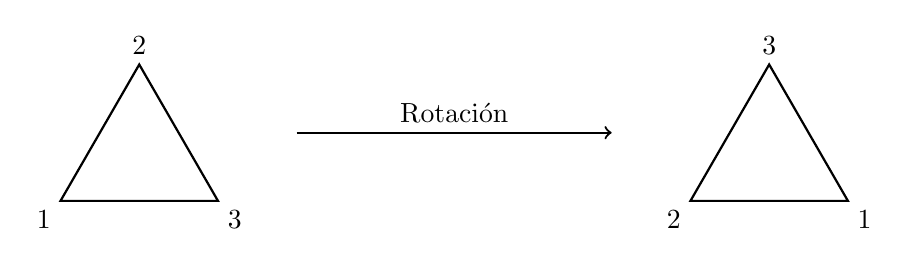
\begin{tikzpicture}
				% Triángulo original
				\draw[thick] (0,0) -- (2,0) -- (1,1.732) -- cycle;
				\node[below left] at (0,0) {1};
				\node[below right] at (2,0) {3};
				\node[above] at (1,1.732) {2};
				
				% Flecha indicando rotación (más grande y centrada)
				\draw[->, thick] (3,0.866) -- (7,0.866) node[midway, above] {Rotación};
				
				% Triángulo con numeración rotada (2,3,1) más separado
				\draw[thick] (8,0) -- (10,0) -- (9,1.732) -- cycle;
				\node[below left] at (8,0) {2};
				\node[below right] at (10,0) {1};
				\node[above] at (9,1.732) {3};
			\end{tikzpicture}
		\end{center}
		
		\medskip
		
		% Segundo diagrama: Reflexión con eje de simetría
		\begin{center}
			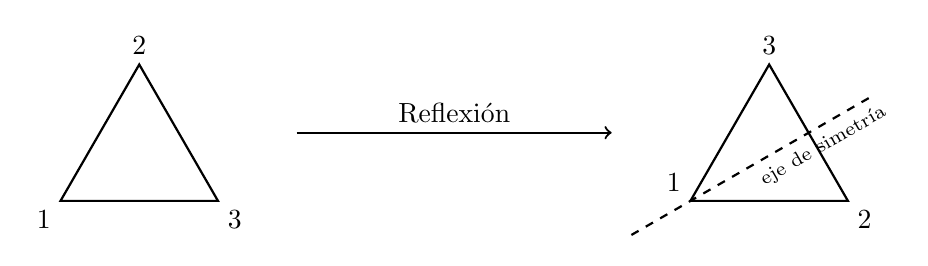
\begin{tikzpicture}
				% Triángulo original
				\draw[thick] (0,0) -- (2,0) -- (1,1.732) -- cycle;
				\node[below left] at (0,0) {1};
				\node[below right] at (2,0) {3};
				\node[above] at (1,1.732) {2};
				
				% Flecha indicando reflexión
				\draw[->, thick] (3,0.866) -- (7,0.866) node[midway, above] {Reflexión};
				
				% Triángulo reflejado con numeración ajustada
				\draw[thick] (8,0) -- (10,0) -- (9,1.732) -- cycle;
				\node[above left] at (8,0) {1};
				\node[below right] at (10,0) {2};
				\node[above] at (9,1.732) {3};
				
				% Eje de simetría (mediana desde vértice 1, extendida simétricamente)
				\draw[dashed, thick] (7.25,-0.433) -- (10.3,1.326) 
				node[pos=0.468, below right, sloped, text depth=0.1ex] 
				{\scriptsize eje de simetría};
			\end{tikzpicture}
		\end{center}
	}
\end{ejemplo}

\vspace{0.5cm}




\begin{proposicion}\label{lkjhgjkl}
	\upshape{
	De la Definción \ref{deiugv} se tiene que 
	\begin{enumerate}
		\item El orden de $\langle a\rangle$ es $n$ y el orden de $\langle b\rangle$ es $2$.
		\item  $b^ra^{s}=a^{-s}b^r$ para todo $r,s\in \mathbb{Z}$ con $r\neq 0$.
		\item $\langle a\rangle$  es un subgrupo normal de $D_n$.
		\item $\langle a \rangle\langle b \rangle=D_n$ y $\langle a \rangle\cap\langle b \rangle=\{I\}$.
	\end{enumerate}
	}
\end{proposicion}

\begin{proof}
	\textcolor{white}{text}
	
	\medskip
	\noindent $[1]$ Como $a$ es un $n$-ciclo, por la Proposición \ref{proppaosjha} tenemos que $a^{\circ n}=I$ y que $a^{\circ(n-1)}\neq I$. Entonces el orden de $a$ es $n$. Así, el orden de $\langle a\rangle$ es $n$. 
	
	\medskip
	\noindent Por otro lado, claramente $b\neq I$ y $b^{\circ 2}=I$. Entonces el orden del subgrupo  $b$ es $2$. Así, el orden de $\langle b\rangle$ es $2$.         \\
	
	\noindent $[2]$ Veamos inicialmente que $ba=a^{-1}b$. En efecto,  
	\[
	ba = \begin{pmatrix}
		1 & 2 & 3 & \cdots & n \\
		1 & n & n-1 & \cdots & 2
	\end{pmatrix}
	(1\ 2\ 3\ \cdots\ n) 
	= \begin{pmatrix}
		1 & 2 & 3 & 4 & \cdots & n-1 & n \\
		n & 1 & 2 & 3 & \cdots & n-2 & n-1
	\end{pmatrix}
	\]     
	
	\[
	a^{-1}b = (n\ n-1\ \cdots\ 2\ 1)\begin{pmatrix}
		1 & 2 & 3 & \cdots & n \\
		1 & n & n-1 & \cdots & 2
	\end{pmatrix} = \begin{pmatrix}
		1 & 2 & 3 & 4 & \cdots & n-1 & n \\
		n & 1 & 2 & 3 & \cdots & n-2 & n-1
	\end{pmatrix}
	\] Así, claramente tenemos que $ba=a^{-1}b$.
	
	\medskip
	\noindent Veamos ahora que $ba^{s}=a^{-s}b$ para todo $s\in \mathbb{Z}$. En efecto:
	\begin{itemize}
		\item Para $s=0$ está claro que es válido.
		\item Es válido para $s\geq 1$: Para $s=1$ hemos visto que es válido. Supongamos que $ba^s=a^{-s}b$ para $s\in \mathbb{N}$ con $s>1$. Entonces $ba^{s+1}=ba^sa=a^{-s}ba=a^{-s}a^{-1}b=a^{-(s+1)}b$.
		\item Es válido para $s\leq -1$: Como $-s\geq 1$ tenemos entonces que $ba^{-s}=a^{-(-s)}b=a^sb$. Entonces $$ba^s=b(a^sb)b=b(ba^{-s})b=a^{-s}b.$$
	\end{itemize}
	\noindent Veamos ahora que dado $s\in \mathbb{Z}$ se cumple que $b^ra^{s}=a^{-s}b^r$ para todo $r\in \mathbb{Z}\setminus\{0\}$. En efecto:
	\begin{itemize}
		\item Es válido para $r\geq 1$: Para $s=1$ hemos visto que es válido. Supongamos que $b^ra^s=a^{-s}b^r$ para $r\in \mathbb{N}$ con $r>1$. Entonces $b^{r+1}a^{s}=bb^ra^s=ba^{-s}b^s=a^{-s}bb^r=a^{-s}b^{r+1}$.
		\item Es válido para $r\leq -1$: Como $-r\geq 1$ tenemos entonces que $b^{-r}a^{s}=a^{-s}b^{-r}$. Entonces \[
		b^r a^{-s} = b^r \left( a^{-s} b^{-r} \right) b^r = b^r \left( b^{-r} a^{s}\right) b^r=a^sb^r.
		\]
		Y como $s\in \mathbb{Z}$ podemos reescribir 
		\[
		b^r a^{s} =a^{-s}b^r.
		\]
	\end{itemize}
	
	
	\noindent $[3]$ Probaremos que $d\langle a\rangle d^{-1}\subset \langle a\rangle$ para todo $d\in D_n$. En efecto:
	\begin{itemize}
		\item Si $d=a^mb^n$:   	
		\begin{align*}
			da^k d^{-1} 
			&= (a^m b^n) a^k (b^{-n} a^{-m}) \\
			&= a^m (b^n a^k) (a^{m} b^{-n}) \\
			&= a^m a^{-k} (b^n a^{m}) b^{-n} \\
			&= a^m a^{-k} a^{-m} b^n b^{-n} \\
			&= a^{-k} \in \langle a \rangle.
		\end{align*}
		
		\item Si $d=b^na^m$: 
		\begin{align*}
			da^k d^{-1} 
			&= (b^n a^m) a^k (a^{-m} b^{-n}) \\
			&= b^na^{k}b^{-n} \\
			&= a^{-k} b^n b^{-n} \\
			&= a^{-k} \in \langle a \rangle.
		\end{align*}
	\end{itemize}    
	Así, tenemos que $\langle a\rangle \trianglelefteq D_n$.\\ 
	
	\noindent $[4]$ En efecto, $\langle a\rangle \langle b \rangle=\{a^{\circ m}b^{\circ n}:m,n\in\mathbb{Z}\}=\langle a,b\rangle=D_n$.
	
	\medskip
	\noindent Por otro lado. Demostremos que $b \notin \langle a \rangle$. Supongamos por contradicción que existe $k \in \mathbb{Z}$ tal que $b = a^k$. Analizando
	\begin{itemize}
		\item Por definición, $b(1) = 1$
		\item $a^k(1) = 1$ solo si:
		\begin{itemize}
			\item Cuando $k = 0$: $a^0 = I$, pero $b \neq I$ pues $b(2) = n \neq 2$
			\item Cuando $k > 0$: $a^k(1) = 1$ implica que $k$ es múltiplo de $n$ (pues $a$ es un $n$-ciclo), luego $a^k = I$, contradicción
			\item Cuando $k < 0$: similarmente lleva a $a^k = I$, contradicción
		\end{itemize}
	\end{itemize}
	Por tanto, no existe tal $k$ y $b \notin \langle a \rangle$. Así $\langle a\rangle \cap \langle b\rangle=\{I\}$.
	
	
\end{proof}

\begin{observacion}
	\upshape{
		De la Proposición \ref{lkjhgjkl} tenemos que $$a^{\circ n}=I ,\qquad b^{\circ 2}=I,\qquad bab=a^{-1}$$
	}
\end{observacion}
Esta observación nos permite dar la presentación del grupo diedral $D_n$.  
\begin{proposicion}
	\upshape{
		El grupo diedral puede escribirse como
		\[
		D_n = \langle x, y : x^n = e,\ y^2 = e,\ yxy = x^{-1} \rangle.
		\]
	}
\end{proposicion}

\begin{proof}[Justificación]
	Consideremos \( X := \{x, y\} \) y definimos una función
	\begin{align*}
		j : X &\longrightarrow D_n \\[4pt]
		x &\longmapsto a \\[2pt]
		y &\longmapsto b
	\end{align*}
	donde \( D_n = \langle a, b \rangle \) que satisfacen:
	\[
	a^n = I,\quad b^2 = I,\quad baba= I.
	\]
	
	\medskip
	
	\noindent Por la propiedad universal del grupo libre, existe un único homomorfismo de grupos
	$f : G_X \longrightarrow D_n$ tal que $f \circ \iota = j$
	\[
	\xymatrix{
		X \ar[rr]^{\displaystyle j} \ar@{^(->}[dd]_{\displaystyle \iota } & & D_n \\ 
		&&\\
		G_X \ar@{-->}[rruu]_{\displaystyle \exists !f} &&
	}
	\] Entonces, el homomorfismo \( f \) se determina en los generadores por:
	\begin{align*}
		f([x]) &= (f\circ\iota)(x)=j(x)=a \\[4pt]
		f([y]) &= (f\circ \iota)(y)=j(y)=b
	\end{align*}
	y, por ser homomorfismo de grupos, se tiene que
	\begin{align*}
		f([x]^n) &= f([x])^n = a^n = I, \\[4pt]
		f([y]^2) &= f([y])^2 = b^2 = I, \\[4pt]
		f([y][x][y][x]) &=f([x])f([y])f([x])f([y]) = abab = I.
	\end{align*}
	Además es un homomorfismo sobreyectivo pues dado $z=a^\alpha b^\beta\in D_n$ existe $[x]^\alpha[y]^\beta\in G_X$ de modo que $f\left([x]^\alpha[y]^\beta\right)=f([x])^\alpha f([y])^\beta=a^\alpha b^\beta=z$.
	
	\medskip
	\noindent
	Definimos el conjunto:
	\[
	R := \{ [x]^n,\ [y]^2,\ [y][x][y][x] \} \subset G_X.
	\] Sea \( N_R \) el subgrupo normal de \( G_X \) generado por \( R \).	Por el teorema fundamental del homomorfismo de grupos, se tiene:
	\[
	G_X / \ker f \cong D_n,
	\]
	Nos interesa saber cómo es el núcleo de $f$. Notemos que $$H:= \langle [x]^n ,\ [y]^2 ,\ [y][x][y][x] \rangle =\ker f.$$ En efecto
	\begin{itemize}
		\item Como los generadores de $H$ se anulan mediante $f$, entonces $H\subset \ker f$.
		\item Notemos primero que como $bab=a^{-1}$ y $b^2=I$, entonces $ba=a^{-1}b$. Sea $w\in \ker f$, entonces existe $k\in \mathbb{N} $ tal que
		\[
		w = [x]^{\alpha_1}[y]^{\beta_1}[x]^{\alpha_2}[y]^{\beta_2} \cdots [x]^{\alpha_k}[y]^{\beta_k}, 
		\quad \text{donde } \alpha_i,\ \beta_i \in \mathbb{Z},\ \text{para } i = 1, \cdots, k
		\] de modo que \[
		f(w) = a^{\alpha_1} b^{\beta_1} a^{\alpha_2} b^{\beta_2} \cdots a^{\alpha_k} b^{\beta_k}=I
		\] Ahora como $ba=a^{-1}b$, entonces $ba^{r}=a^{-r}b$ para todo $r\in \mathbb{Z}$ con lo cual $$b^sa^{r}=a^{-r}b^s,\quad \text{para todo }s,r\in \mathbb{Z}.$$ Entonces
		\[
		f(w) = a^{\alpha_1-\alpha_2-\alpha_3-\cdots-\alpha_k} b^{\beta_1+\beta_2+\cdots+\beta_k}=I
		\]
		Así, \begin{itemize}
			\item $\beta_1+\beta_2+\cdots+\beta_k$ es múltiplo  dos.
			\item $\alpha_1-\alpha_2-\alpha_3-\cdots-\alpha_k$ es múltiplo de $n$. 
			\item 
		\end{itemize}
		
		
	\end{itemize}
	
	
	
	
	
	
	qui
	Debemos probar que $H=\ker f$. La primera inclusión es trivial por lo visto arriba. Sea $w\in \ker(f)$ debemos ver que $w\in H$. En efecto 
	
	
	es un subgrupo normal y por tanto $N_R=H$. En efecto
	
	
	
	
	
	
	
	
	
	
	
	\begin{align*}
		\ker f&=\{\:\xi\in G_X: f\left(\xi\right)=I\:\}\\[4pt]
	\end{align*}
	
	\[
	D_n \cong G_X / N_R = \langle x, y : [x]^n = e,\ [y]^2 = e,\ [y][x][y][x] = e \rangle.
	\]
	
	Finalmente, como las palabras \( [x] \), \( [y] \), \( [x]^n \), etc., están en forma reducida, podemos omitir los corchetes:
	\[
	\langle x, y : [x]^n = e,\ [y]^2 = e,\ [y][x][y][x] = e \rangle = \langle x, y : x^n = e,\ y^2 = e,\ yxy = x^{-1} \rangle.
	\]
\end{proof}









\section{Acción de un grupo}

Sea \( X \) un conjunto no vacío y \( G \) un grupo.

\begin{definicion}
	\upshape{
	Se dice que \( G \) actúa sobre \( X \) si existe una función, denominada \textit{acción de grupo},
	\[
	\varphi : G \times X \to X
	\]
	tal que, para todo \( a, b \in G \) y todo \( x \in X \), se cumplen:
	\begin{enumerate}
		\item Identidad: \( \varphi(e, x) = x \), donde \( e \) es el elemento neutro de \( G \).
		\item Compatibilidad: \( \varphi(ab, x) = \varphi(a, \varphi(b, x)) \).
	\end{enumerate}
	}
\end{definicion}



\begin{observacion}
	\upshape{
		La compatibilidad por sí sola no garantiza que \( \varphi \) sea una acción de grupo: también se requiere la neutralidad.
		
		\medskip
		\noindent Por ejemplo. Sea \( G = (\mathbb{Z}, +) \) y sea \( X = \{a, b\} \). Definimos la aplicación \( \varphi: \mathbb{Z} \times X \to X \) como sigue:
		\[
		\varphi(n, a) = b, \quad \varphi(n, b) = a, \quad \text{para todo } n \in \mathbb{Z}.
		\]
		Es decir, \( \varphi(n, x) \) intercambia \( a \) y \( b \), sin importar el valor de \( n \). Y tenemos
		
		\begin{itemize}
			\item Compatibilidad: Para todo \( n, m \in \mathbb{Z} \) y \( x \in X \), se cumple:			 
			\[
			\varphi(n, \varphi(m, x)) = \varphi(n, y) = x=\varphi(n + m, x),
			\]
			
			\item No se cumple la indentidad. La identidad de \( G \) es \( 0 \), pero:
			\[
			\varphi(0, a) = b \neq a, \quad\text{ y }\quad \varphi(0, b) = a \neq b.
			\]
			Por tanto, la condición $\varphi(e,x)=x$ para todo $x\in X$ falla.
		\end{itemize}
		Concluimos que \( \varphi \) no define una acción de grupo, a pesar de que satisface la compatibilidad.
	}
\end{observacion}




\begin{observacion}\label{hjgfhjkl}
	\upshape{
		Si \( G \) actúa sobre \( X \) mediante \( \varphi \), entonces, para todo \( a \in G \) y \( x \in X \), se cumple:
		\[
		\varphi(a, \varphi(a^{-1}, x)) = x 
		\quad \text{y} \quad 
		\varphi(a^{-1}, \varphi(a, x)) = x.
		\]
		Esto significa que cada aplicación inducida \( \varphi_a : X \to X \), definida por \( \varphi_a(x) := \varphi(a, x) \), es una biyección. Además,
		\[
		\varphi_a^{-1} = \varphi_{a^{-1}}.
		\]
	}
\end{observacion}



\begin{ejemplo}[Acción regular izquierda]
	\upshape{
		Sea \( X = G \). La aplicación \( \varphi(a, x) = ax \) define una acción de \( G \) sobre \( G \).
	}
\end{ejemplo}

\begin{ejemplo}[Acción regular derecha]
	\upshape{
		Sea \( X = G \). No se puede definir la acción como \( \varphi(a, x) = xa \), ya que no cumple la compatibilidad. En su lugar, se define:
		\[
		\varphi(a, x) = x a^{-1},
		\]
		que sí verifica las condiciones de una acción de grupo.
	}
\end{ejemplo}

\begin{ejemplo}[Acción por conjugación]
	\upshape{
		Sea \( X = G \). La aplicación \( \varphi(a, x) = axa^{-1} \) define una acción de \( G \) sobre \( G \) por conjugación.
	}
\end{ejemplo}


\begin{ejemplo}[Acción de traslación]
	\upshape{
		Sea \( G \) un grupo y \( A \) un conjunto. Consideramos el conjunto \( A^G \) de todas las funciones de \( G \) en \( A \). Definimos la aplicación
			\begin{align*}
			\varphi: G\times A^G &\longrightarrow A^G \\[4pt]
			(b,f) &\longmapsto \left(  
			\begin{array}{rcl}
				\varphi(b,f) : G &\to& A \\[2pt]
				x &\mapsto& f(b^{-1}x)
			\end{array} \right)
		\end{align*}
		Esta aplicación define una acción de \( G \) sobre \( A^G \), llamada \emph{acción de traslación (izquierda)}.
	}
\end{ejemplo}



\begin{proposicion}
	\upshape{
		Las siguientes afirmaciones son equivalentes:
		\begin{enumerate}
			\item Toda acción \( \varphi: G \times X \to X \) induce un homomorfismo de grupos \( G \to \operatorname{Biyec}(X) \). Es decir, la aplicación
			\begin{align*}
				\rho: G &\longrightarrow \operatorname{Biyec}(X) \\[4pt]
				a &\longmapsto \left(  
				\begin{array}{rcl}
					\varphi_a : X &\to& X \\[2pt]
					x &\mapsto& \varphi(a, x)
				\end{array} \right)
			\end{align*}
			es un homomorfismo de grupos.
			
			\item Todo homomorfismo de grupos \( \rho: G \to \operatorname{Biyec}(X) \) induce una acción. Es decir, la aplicación 
			\begin{align*}
				\varphi: G \times X &\longrightarrow X\\
				(a,x) &\longmapsto \rho_a(x),
			\end{align*}
			donde \( \rho(a) := \rho_a \in \operatorname{Biyec}(X) \).
		\end{enumerate}
	}
\end{proposicion}


\begin{proof}
	\textcolor{white}{text}
	
	\medskip
	\noindent
	\([1 \Rightarrow 2]\) Supongamos que \( \varphi(ab, x) = \varphi(a, \varphi(b,x)) \) para todo \( a,b \in G \), \( x \in X \).
	
	\medskip
	\noindent 
	Queremos ver que \( \varphi_a \in \operatorname{Biyec}(X) \) para cada \( a \in G \), y que la aplicación
	\[
	\rho : G \to \operatorname{Biyec}(X),\quad a \mapsto \varphi_a,
	\]
	es un homomorfismo de grupos.
	
	\begin{itemize}
		\item Biyectividad: Por la Observación~\ref{hjgfhjkl}, cada \( \varphi_a \) es una biyección con inversa dada por \( \varphi_{a^{-1}} \).
		
		\item Homomorfismo: Para todo \( a,b \in G \) y todo \( x \in X \), se cumple:
		\[
		\varphi_{ab}(x) = \varphi(ab, x) = \varphi(a, \varphi(b, x)) = \varphi_a(\varphi_b(x)) = (\varphi_a \circ \varphi_b)(x).
		\]
		Entonces \( \rho(ab) = \rho(a)\circ\rho(b) \), por lo tanto \( \rho \) es un homomorfismo de grupos.
	\end{itemize}
	
	\medskip
	
	\noindent\([2 \Rightarrow 1]\) Supongamos que \( \rho : G \to \operatorname{Biyec}(X) \), \( a \mapsto \rho_a \), es un homomorfismo de grupos. Entonces, para todo \( a,b \in G \) y \( x \in X \), se cumple:
	\[
	\varphi(ab, x) := \rho_{ab}(x) = (\rho_a \circ \rho_b)(x) = \rho_a(\rho_b(x)) = \varphi(a, \varphi(b, x)),
	\]
	lo que demuestra la compatibilidad. Finalmente, veamos que \( \varphi(e,x) = x \). En efecto, como \( \rho \) es un homomorfismo de grupos, se tiene \( \rho_e = \operatorname{id}_X \), por lo que:
	\[
	\varphi(e,x) = \rho_e(x) = \operatorname{id}_X(x) = x.
	\]
\end{proof}


\begin{observacion}
	\upshape{
		Es usual omitir la notación explícita de la acción \( \varphi: G \times X \to X \) y, en su lugar, denotar simplemente que \( G \) actúa sobre \( X \) escribiendo \( G : X \to X \), y usar la notación \( a \cdot x \) o simplemente \( ax \) para representar la acción de \( a \in G \) sobre \( x \in X \). Con esta convención, las propiedades de la acción se expresan como:
		\[
		a(bx) = (ab)x \quad \text{y} \quad ex = x.
		\]
	}
\end{observacion}
\vspace{0.5cm}

 Cuando \( G \) es un monoide, la acción ya no induce un homomorfismo hacia \( \operatorname{Biyec}(X) \), pues los elementos de \( G \) pueden no ser invertibles. En su lugar, la acción define una aplicación en el monoide de funciones:\[
\operatorname{Fun}(X) := \{ f: X \to X \mid f \text{ es una función} \}.
\]
Con la composición como operación, este conjunto forma un monoide donde las transformaciones no requieren ser biyectivas ni tener inversa.
		
\begin{proposicion}
	\upshape{
		Sea \( M \) un monoide. Son equivalentes:
		\begin{enumerate}
			\item \( M \) actúa sobre \( X \) si existe una función $\varphi : M \times X \to X$ tal que, para todo \( a, b \in M \) y todo \( x \in X \), se cumplen:
			\[
			\varphi(ab, x) = \varphi(a, \varphi(b, x)) \quad\text{ y }\quad \varphi(e, x) = x.
			\]
		
			
			\item \( M \) actúa sobre \( X \) si existe un homomorfismo de monoides $M \to \operatorname{Fun}(X)$.			
			
		\end{enumerate}
	}
\end{proposicion}





\begin{ejemplo}[Aplicación a sistemas dinámicos continuos: Problema de Cauchy]\label{enkbhjgf}
	\upshape{
		Sea \( E \) un espacio de Banach. Sea \( A: E \to E \) un operador cerrado, es decir, una aplicación que lleva conjuntos cerrados en conjuntos cerrados. Considere el problema de Cauchy
		\begin{equation*}
			\left\{
			\begin{aligned}
				u'(t) &= A \cdot u(t), \\
				u(0) &= u_0.
			\end{aligned}
			\right.
		\end{equation*}
		La existencia y unicidad de la solución (global) implica la existencia de una acción del monoide \( (\mathbb{R}_{\geq 0}, +) \), dada por
		\begin{align*}
			\varphi: \mathbb{R}_{\geq 0} \times E &\longrightarrow E \\[4pt]
			(t, u_0) &\longmapsto e^{tA} u_0.
		\end{align*}
	}
\end{ejemplo}


\begin{definicion}
	\upshape{
		Si \( \varphi : G \times X \to X \) es una acción, entonces la \textbf{órbita} de \( x \in X \) es el conjunto
		\[
		G \cdot x := \{ \varphi(a, x) \::\: a \in G \},
		\]
		también denotado por \( \operatorname{Orb}(x) \).
	}
\end{definicion}

\begin{observacion}
	\upshape{
		Obtenemos la misma definición si \( G \) se reemplaza por un monoide \( M \), es decir, si \( \varphi : M \times X \to X \) es una acción de monoide, entonces la órbita de \( x \in X \) se define igual como
		\[
		M \cdot x := \{ \varphi(m, x) \::\: m \in M \},
		\]
		y también se denota por \( \operatorname{Orb}(x) \).
	}
\end{observacion}


\begin{ejemplo}
	\upshape{
		Del Ejemplo \ref{enkbhjgf} (problema de Cauchy), se tiene que
		\[
		\operatorname{Orb}(u_0) = \{ e^{tA} u_0 \::\: t \geq 0 \},
		\]
		esto es, el conjunto de soluciones del sistema dinámico que pasan por \( u_0 \) en \( t = 0 \).
		
		
		
	\begin{center}
		\begin{tikzpicture}[>=Stealth, scale=1.5]
			% Axes
			\draw[->] (-0.5,0) -- (7.5,0) node[right]{$t$};  % Extended x-axis
			\draw[->] (0,-0.5) -- (0,3.5) node[above]{$E$};   % Extended y-axis
			
			% 5 parallel curves (orbits)
			\foreach \y in {0.5,1,1.5,2,2.5} {
				\draw[thick] (0,\y) .. controls (2,\y+0.7) and (5,\y+0.3) .. (7,\y+1);
			}
			
			% Highlighted orbit (u_0)
			\draw[ultra thick] (0,1.5) .. controls (2,2.2) and (5,1.8) .. (7,2.5) 
			node[midway, above left]{$\operatorname{Orb}(u_0)$};
			
			% Initial point
			\filldraw (0,1.5) circle (1.5pt) node[below left]{$u_0$};
		\end{tikzpicture}
	\end{center}
	}
\end{ejemplo}
\begin{ejemplo}[Aplicación a sistemas dinámicos discretos]
	\upshape{
		Sea \( X \) un espacio topológico y definamos
		\[
		\operatorname{Homeo}(X) := \{f : X \to X \mid f \text{ es un homeomorfismo} \}.
		\]
		Sea \( f \in \operatorname{Homeo}(X) \) fijado. Entonces, la aplicación
		\begin{align*}
			\mathbb{Z} &\longrightarrow \operatorname{Homeo}(X) \\[4pt]
			n &\longmapsto f^{\circ n}
		\end{align*}
		define un sistema dinámico discreto con tiempo pasado y futuro. 
		
		\medskip
		\noindent Por otro lado, definamos
		\[
		C^{0}(X) := \{f : X \to X \mid f \text{ es continua} \},
		\]
		entonces la aplicación
		\begin{align*}
			\mathbb{N} &\longrightarrow C^{0}(X) \\[4pt]
			n &\longmapsto f^{\circ n}
		\end{align*}
		define un sistema dinámico discreto con tiempo solo hacia el futuro.
		
		\medskip
		\noindent
		En particular, dado \( z_0 \in \mathbb{C} \), para 
		\begin{align*}
			f : \mathbb{C} &\longrightarrow \mathbb{C} \\[4pt]
			z &\longmapsto z^2 + 1,
		\end{align*}
		tenemos que
		\[
		\operatorname{Orb}(z_0) = \{z_0,\ f(z_0),\ f^{\circ 2}(z_0),\ f^{\circ 3}(z_0),\ f^{\circ 4}(z_0),\ \dots \}.
		\]
		Por ejemplo:
		\begin{equation*}
			\begin{aligned}
				\operatorname{Orb}(i) &= \{ i,\ 0,\ 1,\ 2,\ 5,\ \dots \}, \\[5pt]
				\operatorname{Orb}(i+1) &= \{ i+1,\ 1+2i,\ -2+4i,\ -11-16i,\ \dots \}.
			\end{aligned}
		\end{equation*}
		
	}
\end{ejemplo}

\begin{definicion}
	\upshape{
		Si \( \varphi : G \times X \to X \) es una acción, entonces el \textit{estabilizador} de \( x \in X \) es el conjunto
		\[
		\operatorname{Stab}(x) := \{ a \in G : \varphi(a, x) = x \}.
		\]
	}
\end{definicion}

\begin{proposicion}
	\upshape{
		Para cualquier \( x \in X \), el conjunto \( \operatorname{Stab}(x) \) es un subgrupo de \( G \).
	}
\end{proposicion}

\begin{proof}
	Dado $x\in X$. Sean $a,b\in \operatorname{Stab}(x)$ entonces $\varphi(a,x)=x$ y $\varphi(b,x)=x$. Entonces $$\varphi(ab^{-1},x)=\varphi\left(a,\varphi(b^{-1},x)\right)=\varphi\left(a,\varphi(b^{-1},\varphi(b,x))\right)=\varphi\left(a,\varphi(e,x)\right)=\varphi(a,x)=x.$$Por tanto, \( ab^{-1} \in \operatorname{Stab}(x) \), lo que demuestra que \( \operatorname{Stab}(x) \) es un subgrupo de \( G \).
\end{proof}



